% --------------------------------------------------------------------------- %
% --------------------------------------------------------------------------- %
\chapter{Theory and Motivation}
\label{ch:intro}

Particle physics is concerned with the study of the most fundamental constituents of nature and the rules that govern their interactions. Over the course of the twentieth century, physicists developed models using quantum field theory to describe the fundamental forces binding elementary particles together, and experimentalists discovered an abundance of particles predicted by such theories. Today, the Standard Model of particle physics represents the best experimental verified theoretical framework for describing the elementary components of the universe, and experimental particle physicists work in tandem with theorists to identify possible extensions to the Standard Model which may explain some theoretical and experimental issues with the current framework.

\section{The Standard Model of Particle Physics}
\label{sec:sm}

The Standard Model (SM) is a quantum field theory which describes the fundamental particles which make up the universe and the various interactions between those particles. It is widely regarded as one of the most successful theories ever constructed to describe nature, and has been rigorously verified experimentally. The announcement in 2012 by the ATLAS and CMS detectors of a new particle consistent with the Higgs Boson marked the discovery of the last fundamental particle predicted by the SM over 50 years before its discovery, and many precision measurements of the Standard model parameters have been verified to better than one part in a billion.

The SM classifies all the elementary particles into two categories, depending on their intrinsic angular momentum, {\it spin}. Particles with a half-integer spin are known as {\it fermions} while those with integer spin are referred to as {\it bosons}. Fermions obey the Pauli exclusion principle (where identical fermions cannot occupy the same quantum state), and are often thought of as the constituents of matter. Bosons are not subject to the Pauli exclusion principle, and are often thought of as the ``force carriers'' which mediate different fundamental forces between different particles. The various fundamental particles of the SM and their properties are detailed in figure \ref{fig:sm}.

Fermions can be divided into two groups, {\it leptons} and {\it quarks}. Both leptons and quarks can be further divided into two subgroups based on their electromagnetic charge. Charged leptons carry either positive or negative charge {\it e} (where {\it e} is the fundamental charge constant), whereas the neutral leptons known as {\it neutrinos} carry no electromagnetic charge. Different species of quarks can be either positively charged (+2/3{\it e}) or negatively charged (-1/3{\it e}). Both leptons and quarks can also be divided into three ``flavors'' of particles grouped into different families with similar electromagnetic properties but different masses. The leptons in order of increasing mass are {\it electron}, {\it muon}, or {\it tau} flavored (with both charged lepton and neutrino species), and the quarks are grouped into {\it up/down}, {\it charmed/strange}, and {\it top/bottom} pairs (that are positively and negatively charged, respectively).

The bosons of the standard model are associated with the different fundamental forces by which particles (including the bosons themselves) interact. The Standard Model Lagrangian is invariant under local transformations of an $SU(3) \times SU(2) \times U(1)$ gauge symmetry, and the various gauge symmetries correspond to different forces through which particles interact. $SU(3)$ is associated with the Quantum Chromodynamics (QCD) color charge (or strong force), and mediated by the {\it gluon} which binds quarks together (leptons are represented by an $SU(3)$ singlet and do not interact via the strong force). The $SU(2) \times U(1)$ groups are associated with weak isospin and hypercharge respectively, and responsible for electroweak interactions between particles, mediated by the {\it $W^\pm$} and {\it Z} bosons and the {\it photon}, $\gamma$.

While the gauge symmetries of the standard model are preserved, explicit mass terms are forbidden in the Lagrangian and the associated gauge bosons might otherwise remain massless. However, the SM Lagrangian also includes a complex scalar doublet which allows for the Higgs mechanism; the neutral component of the scalar doublet acquires a non-zero vacuum expectation value which manifests as the {\it Higgs boson}, and the other degrees of freedom become Goldstone bosons which grant mass to the {\it $W^\pm$} and {\it Z} bosons. In this manner the electroweak $SU(2) \times U(1)$ is spontaneously broken into the familiar weak and electromagnetic forces.

\begin{figure}
	\centering
	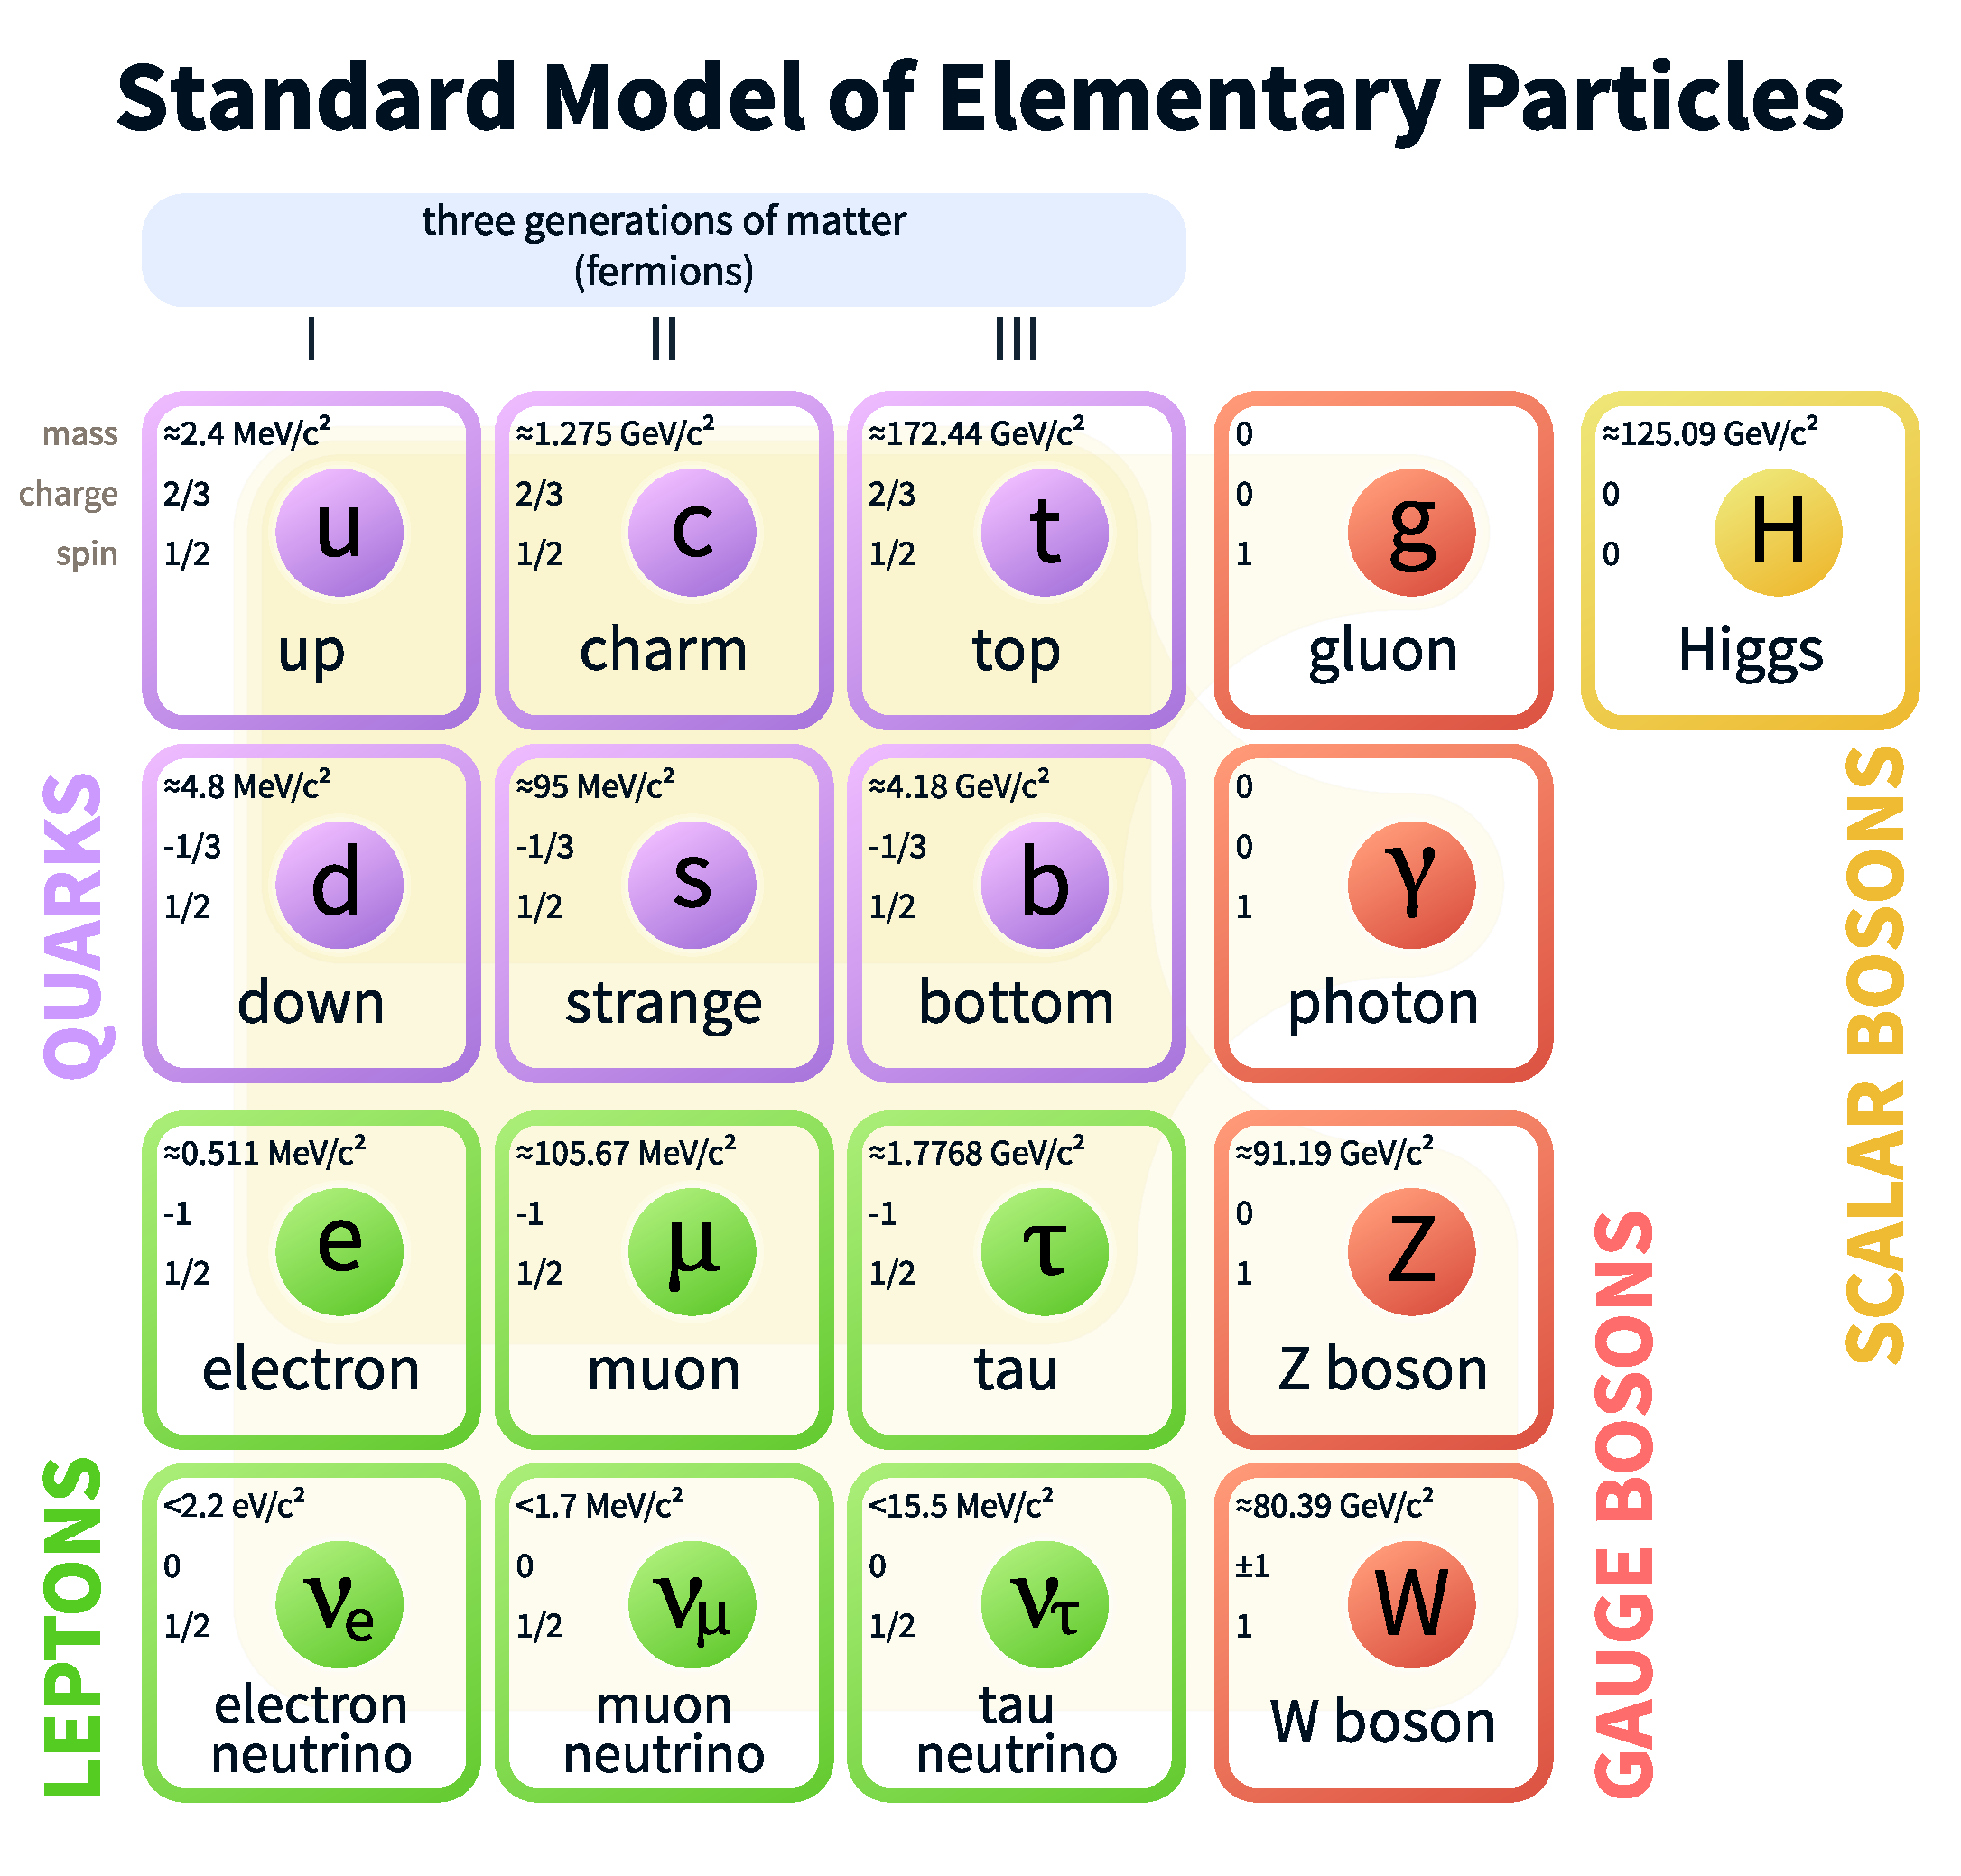
\includegraphics[width=0.9\textwidth]{intro/figs/Standard_Model_of_Elementary_Particles}
	\caption{An illustration of the elementary particles in the Standard Model and their properties. The three left columns represent the different generations of fermions, with quarks in purple and leptons in green. The gauge bosons are represented in the fourth column in red, and the only scalar boson, the Higgs, in the fifth column in yellow. \cite{cc}}
	\label{fig:sm}
\end{figure}

\section{Issues with the Standard Model}
\label{sec:smIssues}

Despite the great success of the Standard Model in describing many of the fundamental interactions of particles, it is insufficient to explain all physical phenomena. There are several outstanding theoretical questions left unanswered by the Standard Model, and experimental evidence to suggest it is incomplete.

One of the most perplexing theoretical features of the SM is the fact that we have been able to detect all the elementary particles at energies accessible in our experiments. Because the bare masses of particles in the SM Lagrangian receive corrections from quantum loop diagrams, it is not clear why new particles (which must be massive) do not contribute significantly to these corrections. In particular, the quantum loop corrections to the Higgs boson mass include all massive particles, and contributions from undiscovered massive particles could drive the Higgs mass far beyond what is currently accessible, yet this is not observed. This is often referred to as the {\it hierarchy problem}.

Experimental evidence also suggests there are physical phenomena not explained by the SM. Measurements of the rotational velocity of galaxies compared to the visible matter indicate there is an abundance of {\it dark matter} in the universe which cannot be accounted for by the particle content of the SM. Furthermore, while the SM predicts neutrinos to be massless, measurements of neutrino flavor oscillations imply that neutrinos mass is very small, but nonzero. Such measured phenomena indicate there may be additional particle content beyond what is posited by the SM, and additional interaction terms between SM particles and a ``dark sector'' of weakly-interacting particles.

\section{Beyond the Standard Model: Supersymmetry}
\label{sec:bsm}

In order to solve many of the theoretical and experimental issues with the SM, theorists had considered extending SM particle content and interactions to include additional species which might satisfy some of the theoretical constraints of the SM in a consistent manner with observation. However, in 1975 the Haag??opusza?ski?Sohnius theorem demonstrated that the only non-trivial extensions of quantum theories do not only include internal symmetries and the Poincar� symmetry, but also a non-trivial extension of the Poincar� algebra known as {\it supersymmetry}.

A quantum field theory of supersymmetry (SUSY) can be visualized as a dual version of a typical field theory. For each particle, there exists a superpartner with different spin; fermions have boson-like superpartners and bosons have fermion-like superpartners. This is a particularly appealing and elegant solution to many of the issues with the SM; loop diagram corrections to particle mass are partially cancelled out by contributions from superpartner loop diagrams, providing a natural solution to the hierarchy problem. In typical ``R-parity conserving'' SUSY theories, particle interactions also conserve ``SUSY-ness'' in decays, and thus when a superparticle decays into SM particles, the cascade will always end in the lightest supersymmetric particle (LSP). The LSP must be stable, and because it interacts very weakly with the SM sector provides a suitable dark matter candidate.

While there are many beyond-SM (BSM) theories that seek to explain phenomena beyond the scope of the SM, SUSY provides both elegant solutions to the theoretical concerns of the SM as well as a robust framework to unexplained physical phenomena. The analysis described here is designed to be model independent in a search for new physics, but also sets constraints on SUSY models as it is one of the most promising BSM theories that might be realized by nature.
% --------------------------------------------------------------------------- %
% --------------------------------------------------------------------------- %
